\chapter{System Design and modelling}

This chapter presents comprehensive architectural models and design documentation for Ather Co-Pilot, using industry-standard notation and visualization techniques. The models below collectively describe system requirements, temporal planning, data movement, control logic, user interactions, workflow sequences, and persistent data structures.

\section{Gnatt Chart}
A Gantt chart is a type of bar chart that illustrates a project schedule. It provides a visual timeline for tasks to be performed, showing the start and finish dates of the terminal elements and summary elements of a project. For Aether Co-Pilot, the Gantt chart maps out the 16-week development lifecycle, highlighting the critical paths between Requirement Analysis, System Design, Frontend/Backend Integration, and Final deployment.

\begin{center}
\vspace{0.05cm}
\resizebox{\textwidth}{!}{%
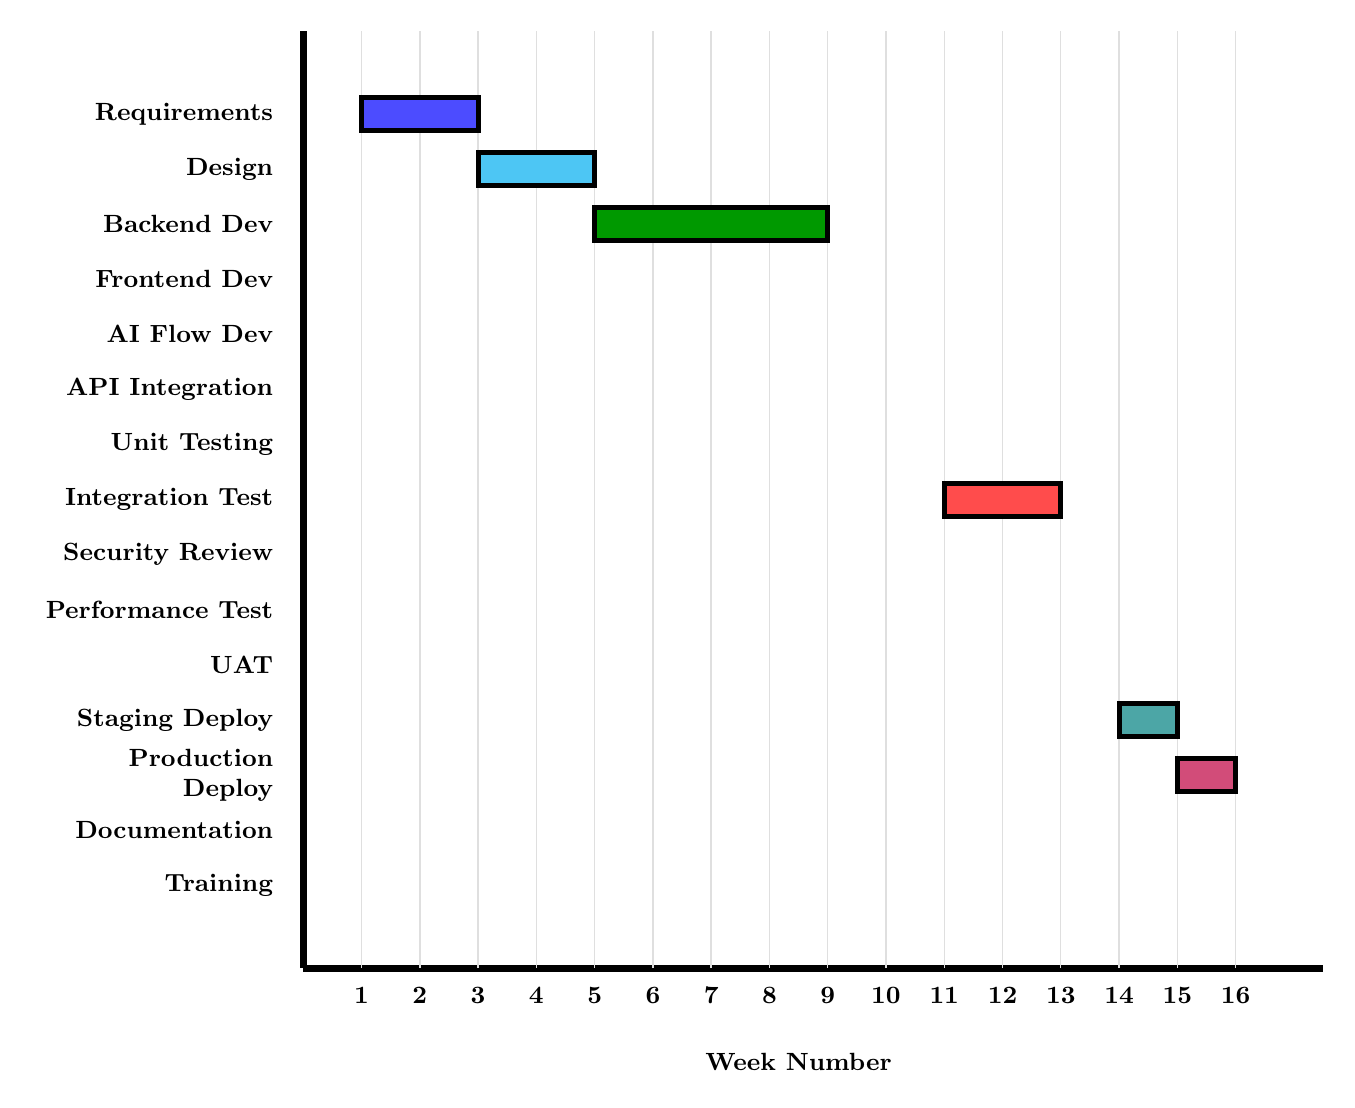
\begin{tikzpicture}[
    x=0.74cm, y=0.70cm,
    font=\sffamily,
    task/.style={font=\bfseries\small, anchor=east, text width=3.0cm, align=right},
    week_header/.style={font=\bfseries\small},
    bar_label/.style={font=\bfseries\tiny, color=white},
    milestone/.style={circle, draw=black, line width=0.6pt, font=\bfseries\small, inner sep=3.5pt, text=white},
    crit_path/.style={draw=black, line width=1.8pt},
    parallel_path/.style={draw=black, line width=1pt},
    dependency/.style={->, line width=1.4pt, color=gray!75, shorten >=2pt, shorten <=2pt}
]
% AXES & GRID
\draw[line width=2.5pt] (0,0.5) -- (17.5,0.5); % X-axis
\draw[line width=2.5pt] (0,0.5) -- (0,17.5);   % Y-axis
\foreach \x in {1,...,16} {
    \draw[gray!25, line width=0.5pt] (\x,0.5) -- (\x,17.5);
    \node[week_header] at (\x,0) {\x};
}
\node[font=\bfseries\small] at (8.5, -1.2) {Week Number};

% TASK LABELS
\node[task] at (-0.35,16) {Requirements};
\node[task] at (-0.35,15) {Design};
\node[task] at (-0.35,14) {Backend Dev};
\node[task] at (-0.35,13) {Frontend Dev};
\node[task] at (-0.35,12) {AI Flow Dev};
\node[task] at (-0.35,11) {API Integration};
\node[task] at (-0.35,10) {Unit Testing};
\node[task] at (-0.35,9) {Integration Test};
\node[task] at (-0.35,8) {Security Review};
\node[task] at (-0.35,7) {Performance Test};
\node[task] at (-0.35,6) {UAT};
\node[task] at (-0.35,5) {Staging Deploy};
\node[task] at (-0.35,4) {Production Deploy};
\node[task] at (-0.35,3) {Documentation};
\node[task] at (-0.35,2) {Training};

% BARS
\fill[crit_path, fill=blue!70] (1,15.7) rectangle (3,16.3); 
\fill[crit_path, fill=cyan!70] (3,14.7) rectangle (5,15.3); 
\fill[crit_path, fill=green!60!black] (5,13.7) rectangle (9,14.3); 
\fill[crit_path, fill=red!70] (11,8.7) rectangle (13,9.3); 
\fill[crit_path, fill=teal!70] (14,4.7) rectangle (15,5.3); 
\fill[crit_path, fill=purple!70] (15,3.7) rectangle (16,4.3); 

\end{tikzpicture}%
}
\captionof{figure}{Project Gantt Chart Timeline}
\end{center}

\clearpage

\section{DFD}
A Data Flow Diagram (DFD) maps out the flow of information for any process or system. It uses defined symbols like rectangles, circles and arrows to show data inputs, outputs, storage points and the routes between each destination. In Aether Co-Pilot, the level-0 DFD illustrates the macroscopic data exchange from the user, through our API layer, into the Gemini model, and finally recording state in the Firestore DB.

\begin{center}
\vspace{0.15cm}
\resizebox{0.75\textwidth}{!}{%
\begin{tikzpicture}[>=latex, node distance=1.65cm, auto, thick, font=\small,
    ext/.style={draw, rectangle, minimum width=2.2cm, minimum height=0.75cm, align=center, fill=yellow!15},
    proc/.style={draw, circle, minimum size=1.65cm, align=center, fill=cyan!15},
    store/.style={draw, rectangle, minimum width=2.2cm, minimum height=0.75cm, align=center, fill=gray!15}]

\node[ext] (user) {User};
\node[proc, right=of user, xshift=0.15cm] (system) {Ather\\Co-Pilot};
\node[ext, right=of system, xshift=0.15cm] (gemini) {Gemini};
\node[store, below=of system, yshift=-0.2cm] (db) {Firestore};

\draw[line width=1.2pt] (user) -- (system) node[midway, above, font=\tiny] {Prompt};
\draw[line width=1.2pt] (system) -- (gemini) node[midway, above, font=\tiny] {Infer};
\draw[line width=1.2pt] (gemini) -- (system);
\draw[line width=1.2pt] (system) -- (user) node[midway, below, font=\tiny] {Response};
\draw[line width=1.2pt] (system) -- (db) node[midway, right, font=\tiny] {History};
\end{tikzpicture}%
}
\captionof{figure}{Level-0 DFD: Core System Data Movement}
\end{center}

\clearpage

\section{Flow Diagram}
A Flow Diagram is a graphical representation of a process, depicting the sequential steps required to solve a problem or handle a routine. The primary control flow for Aether Co-Pilot enforces security checks. It visualizes how an incoming prompt immediately encounters an authentication gate, blocking invalid requests, before advancing to prompt generation and history logging.

\begin{center}
\vspace{0.15cm}
\resizebox{0.72\textwidth}{!}{%
\begin{tikzpicture}[>=latex, node distance=1.15cm, auto, thick, font=\small,
    startstop/.style={draw, rounded corners, minimum width=2.7cm, minimum height=0.72cm, align=center, fill=yellow!20},
    proc/.style={draw, rectangle, minimum width=3.3cm, minimum height=0.72cm, align=center, fill=green!10},
    decision/.style={draw, diamond, aspect=1.8, align=center, inner sep=1pt, fill=red!10}]

\node[startstop] (start) {Start};
\node[proc, below=of start] (receive) {Receive Request};
\node[decision, below=of receive, yshift=-0.15cm] (auth) {Authenticated?};
\node[proc, below left=1.1cm and 1.6cm of auth] (deny) {Deny \& Redirect};
\node[proc, below right=1.1cm and 1.6cm of auth] (gen) {Generate Response};
\node[startstop, below=of gen] (end) {Send \& Log};

\draw[line width=1.2pt] (start) -- (receive);
\draw[line width=1.2pt] (receive) -- (auth);
\draw[line width=1.2pt] (auth) -- node[left, font=\tiny] {No} (deny);
\draw[line width=1.2pt] (auth) -- node[right, font=\tiny] {Yes} (gen);
\draw[line width=1.2pt] (gen) -- (end);
\end{tikzpicture}%
}
\captionof{figure}{Control Flow: Request Handling with Security}
\end{center}

\clearpage

\section{Use Case diagram}
A Use Case diagram captures the dynamic behavior of a live system. It models the functionality of a system using actors and use cases, showing what tasks the system performs for the users. Here, the authenticated user actor interacts with four primary use cases: Chat Initiation, Code Generation, Material Upload, and Task creation workflows.

\begin{center}
\vspace{0.15cm}
\resizebox{0.82\textwidth}{!}{%
\begin{tikzpicture}[>=latex, node distance=1.1cm, auto, thick, font=\small,
    actor/.style={draw, rectangle, rounded corners, minimum width=2.0cm, minimum height=0.65cm, align=center, fill=blue!15},
    usecase/.style={draw, ellipse, minimum width=3.1cm, minimum height=0.77cm, align=center, fill=green!10},
    boundary/.style={draw, dashed, line width=1.2pt, minimum width=7.2cm, minimum height=4.8cm}]

\node[actor] (user) at (-3.7,1.55) {Authenticated\\User};
\node[boundary, anchor=north west] (sys) at (-1.6,3.0) {};
\node[font=\small\bfseries] at (1.6,2.75) {Aether Co-Pilot};

\node[usecase] (uc1) at (1.6,1.85) {Initiate Chat};
\node[usecase] (uc2) at (1.6,1.0) {Generate Code};
\node[usecase] (uc3) at (1.6,0.15) {Upload Material};
\node[usecase] (uc4) at (1.6,-0.7) {Create Task};

\draw[line width=1pt] (user) -- (uc1);
\draw[line width=1pt] (user) -- (uc2);
\draw[line width=1pt] (user) -- (uc3);
\draw[line width=1pt] (user) -- (uc4);
\end{tikzpicture}%
}
\captionof{figure}{Use Case Diagram: Core Functionalities}
\end{center}

\clearpage

\section{Activity diagram}
An Activity Diagram is basically a flowchart to represent the flow from one activity to another activity. The activity can be described as an operation of the system. For Aether, it maps the chat request processing workflow, showcasing decision points like validating the user's session context against the backend and handling potential error conditions elegantly.

\begin{center}
\vspace{0.12cm}
\resizebox{0.70\textwidth}{!}{%
\begin{tikzpicture}[>=latex, node distance=1.1cm, auto, thick, font=\small,
    action/.style={draw, rectangle, minimum width=3.2cm, minimum height=0.70cm, align=center, fill=green!10},
    decision/.style={draw, diamond, aspect=1.8, align=center, inner sep=1pt, fill=red!10}]

\node[circle, draw, fill=black, minimum size=0.23cm, inner sep=0pt] (start) {};
\node[action, below=of start] (input) {Enter Prompt};
\node[action, below=of input] (validate) {Validate Session};
\node[decision, below=of validate, yshift=-0.12cm] (ok) {Valid?};
\node[action, below left=1.05cm and 1.45cm of ok, font=\small] (retry) {Show Error};
\node[action, below right=1.05cm and 1.45cm of ok] (call) {Call Gemini};
\node[action, below=of call] (render) {Render \& Save};
\node[circle, draw, fill=black, minimum size=0.23cm, inner sep=0pt, below=of render] (end) {};

\draw[line width=1.1pt] (start) -- (input);
\draw[line width=1.1pt] (input) -- (validate);
\draw[line width=1.1pt] (validate) -- (ok);
\draw[line width=1.1pt] (ok) -- node[left, font=\tiny] {No} (retry);
\draw[line width=1.1pt] (ok) -- node[right, font=\tiny] {Yes} (call);
\draw[line width=1.1pt] (call) -- (render);
\draw[line width=1.1pt] (render) -- (end);
\end{tikzpicture}%
}
\captionof{figure}{Activity Diagram: Request Processing Workflow}
\end{center}

\clearpage

\section{ER diagram}
An Entity Relationship Diagram (ERD) illustrates how entities such as databases, objects, or systems relate to one another within a system. This diagram maps out our NoSQL Firestore schema hierarchy. It establishes the central USER entity, displaying 1-to-many relationships branching out towards SESSION sub-collections, MESSAGE sub-collections, and standalone SNIPPETS.

\begin{center}
\vspace{0.15cm}
\resizebox{0.75\textwidth}{!}{%
\begin{tikzpicture}[>=latex, node distance=1.6cm, auto, thick, font=\small,
    entity/.style={draw, rectangle, minimum width=2.4cm, minimum height=0.75cm, align=center, fill=cyan!15}]

\node[entity] (user) {USER\\{\tiny userId, email}};
\node[entity, right=of user, xshift=0.65cm] (session) {SESSION\\{\tiny sessionId, title}};
\node[entity, below=of session, yshift=0cm] (message) {MESSAGE\\{\tiny msgId, role}};
\node[entity, below=of user, yshift=0cm] (snippet) {SNIPPET\\{\tiny snippetId, type}};

\draw[line width=1.2pt, ->] (user) -- node[above, font=\tiny\bfseries] {1:N} (session);
\draw[line width=1.2pt, ->] (session) -- node[right, font=\tiny\bfseries] {1:N} (message);
\draw[line width=1.2pt, ->] (user) -- node[left, font=\tiny\bfseries] {1:N} (snippet);
\end{tikzpicture}%
}
\captionof{figure}{Entity-Relationship Diagram}
\end{center}

\newpage
